\documentclass[12pt, letterpaper, titlepage]{article}

\usepackage{amsmath}
\usepackage{amssymb}
\usepackage{booktabs}
\usepackage{amsthm}
\usepackage{graphicx}
\usepackage[margin=1in]{geometry}
\usepackage{hyperref, url}
\hypersetup{colorlinks = true, linkcolor = blue, citecolor=blue, urlcolor =
  blue}
\usepackage{natbib}
\usepackage{enumitem}
\usepackage{setspace}

\usepackage[pagewise]{lineno}
%\linenumbers*[1]
% %% patches to make lineno work better with amsmath
\newcommand*\patchAmsMathEnvironmentForLineno[1]{%
 \expandafter\let\csname old#1\expandafter\endcsname\csname #1\endcsname
 \expandafter\let\csname oldend#1\expandafter\endcsname\csname end#1\endcsname
 \renewenvironment{#1}%
 {\linenomath\csname old#1\endcsname}%
 {\csname oldend#1\endcsname\endlinenomath}}%
\newcommand*\patchBothAmsMathEnvironmentsForLineno[1]{%
 \patchAmsMathEnvironmentForLineno{#1}%
 \patchAmsMathEnvironmentForLineno{#1*}}%

\AtBeginDocument{%
 \patchBothAmsMathEnvironmentsForLineno{equation}%
 \patchBothAmsMathEnvironmentsForLineno{align}%
 \patchBothAmsMathEnvironmentsForLineno{flalign}%
 \patchBothAmsMathEnvironmentsForLineno{alignat}%
 \patchBothAmsMathEnvironmentsForLineno{gather}%
 \patchBothAmsMathEnvironmentsForLineno{multline}%
}

% control floats
\renewcommand\floatpagefraction{.9}
\renewcommand\topfraction{.9}
\renewcommand\bottomfraction{.9}
\renewcommand\textfraction{.1}
\setcounter{totalnumber}{50}
\setcounter{topnumber}{50}
\setcounter{bottomnumber}{50}

\newcommand{\jy}[1]{\textcolor{blue}{JY: #1}}
\newcommand{\eds}[1]{\textcolor{red}{EDS: (#1)}}


\title{On Sample Size for Block Bootstrap Confidence Intervals 
  to Have Desired Coverage Rates}

\author{Mathew Chandy
%   \href{mailto:mathew.chandy@uconn.edu}
% {\nolinkurl{mathew.chandy@uconn.edu}}\\
  and Jun Yan\\[1ex]
  Department of Statistics, University of Connecticut\\
}
\date{}

\begin{document} 
\maketitle

\begin{abstract}
Block bootstrap is a method that is useful for estimating a parameter of a time
series. Theoretically, the method will work perfectly given an infinitely
large sample of the time series. It is necessary to know how large of a finite
sample is required for block bootstrap estimation to work. Before this study,
there have been no investigations into this problem within the literature. The
aim of this study is to answer this question by simulating replications of
block bootstrap interval estimations of a parameter of a time series, and
recording the rate at which the parameter is recovered by each replicate
interval. The sample length required for acceptable performance is
unsurprisingly found to be dependent on the type of interval construction and
the series' level of temporal dependence.


\bigskip
\noindent{\sc Keywords}:
dependent data; gsimulation
\end{abstract}

\doublespace

\jy{Practice my writing tips on latex (e.g., keep line width under 80; use
  double blank lines to separate paragraphs; etc.):
  \url{
https://statds.github.io/stat-writing/using-the-right-tools-for-writing.html},
  chapter 2}


\section{Introduction}
\label{sec:intro}

Block bootstrap is a powerful tool for constructing confidence intervals (CI)
when making inferences about dependent data. Early ideas were developed
independently by \citet{hall1985resampling}, \citet{carlstein1986use}, and 
\citet{kunsch1989jackknife}.
It has since been applied in various fields such as econometrics
\citep{mackinnon2006bootstrap} and meteorology \citep{varga2017generalised}.
Block bootstrap is particularly useful for serially dependent
data when the serial dependence is not specified or not of primary interest.
The method is expected to produce CIs with coverage rates
matching their nominal levels as the sample size grows to infinity. However,
when dealing with finite sample sizes, an important question is how large the
sample size needs to be for block bootstrap CIs to have the
desired coverage rates.


The necessary sample size for bootstrap standard errors to provide valid
uncertainty measures in practice has not been extensively studied. For
independent data and non-block bootstrap, \citet{hesterberg2015teachers} notes
that while percentile-based CIs from nonparametric bootstrap
are more accurate than $t$-intervals for larger sample sizes, they are
less accurate for smaller sample sizes. In the contect of structural equation
modeling, \citet{nevitt2001performance} find
that a sample size of 200--1000 is usually sufficient for interval estimation
using standard nonparametric bootstrap. For dependent data, the necessary sample
size for block bootstrap is even less clear. In a linear regression setting with
dependent data, \citet{goncalves2005bootstrap} find that, standard error
estimates from block bootstrap in small samples may be more accurate than
inference from closed-form asymptotic estimates, but block bootstrap percentile
CIs still do not have sufficient coverage even for sample size
$n = 1024$.


The goal of this paper is to provide some practical recommendations on
necessary sample size for block bootstrap with dependent data. We consider a
simple situation of a stationary time series, where the parameters of
interests are the mean, standard deviation, and the first-order
autocorrelation coefficient. We compare three variants of block bootstrap
CIs from the literature \citep{diciccio1996bootstrap,
  rice2006mathematical}: a basic percentile interval, a percentile
interval centered around the estimate, and a bias-corrected and
accelerated ($BC_a$) interval also centered around the original estimate. Their
empirical coverage rates at different sample sizes and dependence levels are
compared in a simulation study. The results of this study suggest that
appropriate recovery of temporal dependence parameters is heavily dependent on
the type of interval used.


The remainder of the papers is organized as follows:
The Block Bootstrap CIs section reviews how these intervals
are constructed as well as the general procedure for block bootstrap parameter
estimation. The Simulation Study section offers an explanation of the
simulation design and results. Finally, the Concluding Remarks section
discusses the main takeaways from the results, how these findings could be
useful, and possible future explorations.


\section{Block Bootstrap CIs}
\label{sec:blkbootreview}

Consider a stationary time series $\{X_t: t = 1, \ldots, n\}$ with length~$n$.
Our goal is to construct a CIs for a parameter $\theta$ in the
data generating model of the series. Suppose that $\hat\theta_n$ is a point
estimator of~$\theta$ based on the observed series. Bootstrap is a powerful
approach to construct CIs. If the observations in the series
were independent, a standard nonparametric bootstrap procedure would draw a
large number~$B$ bootstrap copies of the observed data, and calculate an
estimate $\hat\theta_n^{(b)}$ for each copy $b = 1, \ldots, B$. The uncertainty
of $\hat\theta_n$ is then estimated by the empirical uncertainty of the
$\hat\theta_n^{(b)}$'s. When serial dependence is present, the bootstrap
procedure needs to preserve the serial dependence. Block bootstrap was
motivated for this situation. 


\subsection{Block Bootstrap Sample}

Block bootstrap preserves the serial dependence in the observed data by
partitioning the data into blocks and perform bootstrap on the blocks.
In particular, consider block size~$l$ and, for convenience, suppose that
$n$ is a multiple of $l$ such that there are $k = n / l$ blocks. Each block~$j$
is $Y_j = \{X_{(j - 1) * l + 1}, \ldots, X_{(j - 1) * l + l}\}$,
$j = 1, \ldots,   k$.  Then, we sample $k$ blocks of $Y_j$'s from the set 
$\{Y_1, \ldots, Y_k\}$ with replacement and concatenate the $k$ sampled blocks
in the order they are picked to form a bootstrap sample of the data. The
formation of the bootstrap sample ensures that the between-block dependence is
week and that the within-block serial dependence is preserved. Because the
blocks here are non-overlapping, this bootstrap approach is known as
non-overlapping block bootstrap, or simple block bootstrap.


Alternatively, block-bootstrap can be done with overlapping or moving blocks.
Define moving blocks $Z_j = \{X_j, \ldots, X_{j + l - 1}\}$,
$j = 1, \ldots, n - l + 1$. Now we draw $k$ blocks from the $(n - l + 1)$
blocks
of $Z_j$'s with replacement and then aligning them in the order they were
picked
to form a block bootstrap sample. If $n$ is not a multiple of~$l$, the last
block selected will be reduced in size so that the final size of the
block bootstrap sample is $n$. It is also possible to implement moving block
bootstrap while allowing blocks to wrap around the end of the series. In other
words, define moving blocks (assuming $l > 1$):



\begin{equation}
Z_j =
    \begin{cases}
        \{X_j, \ldots, X_{j + l - 1}\} & \text{if } j = 1, \dots, n - l + 1\\
        \{X_j, \ldots, X_n, X_1, \ldots, X_{l - 1}\} & \text{if } j = n - l + 2 ,\dots, n
    \end{cases}
\end{equation}

The second implementation of moving block bootstrap was used in
this study, and moving block bootstrap in general had been found to yield the 
lowest error.
\citep{radovanov2014comparison}.  
\jy{what does the last sentence mean?} Addressed


The block size~$l$ needs to chosen with care. It needs to be large enough for
each bootstrap sample to preserve the serial dependence, yet small enough for
there to be some variability between each bootstrap sample. As $n$ increases,
$l$ should also increase, but $l / n$ should decrease. To achieve this, $l$ is
often assigned a value as a function of $n$. A common function that is
considered the best by much previous literature is $l = \lceil n^{1/3} \rceil$
\citep{buhlmann1999block}.


\subsection{Construct CIs}

Suppose that we have repeated the steps in the last subsection $B$ times, and
that for $b \in \{1, \ldots, B\}$, we have obtained an estimator
$\hat\theta_n^{(b)}$ based on the $b$th bootstrap sample using the same method
that was applied to $\{X_t: t = 1, \ldots, n\}$ to obtain $\hat\theta_n$.
Now the question is, how to construct CIs for $\theta$
using the $B$ bootstrap point estimates
$\{\hat\theta_n^{(1)}, \ldots, \hat\theta_n^{(B)}\}$.
We consider three kinds of CIs.


\paragraph{Percentile CI}
Let $\hat\theta_{n, \alpha}^{(b)}$ be the empirical $100\alpha$th percentile of
$\{\hat\theta_n^{(1)}, \ldots, \hat\theta_n^{(B)}\}$. The $(1 - \alpha)$
empirical percentile CI is
\[
(\hat\theta_{n, \alpha/2}^{(b)}, \hat\theta_{n, 1 - \alpha/2}^{(b)}).
\]
This CI is not necessarily centered by the point estimator $\hat\theta_n$.
%% Not the right place
%% This interval works well when attempting to recover the mean and
%% standard deviation of a temporally dependent process, but its coverage of
%% the temporal dependence deteriorates as $n$ increases.


\paragraph{Centered Percentile CI}
Centered percentile CI is centered at the point estimator and uses the
variation
in the bootstrap estimates to construct the error bound. This interval requires
the computation of $\bar\theta_n^{(b)}$, the mean of all bootstrap point
estimates, and $\delta$, the difference between a point estimate and
$\bar\theta_n^{(b)}$. For $b \in \{1, \ldots, B\}$, we can obtain a
$\delta^{(b)}$ based on the $b$th bootstrap point estimate. Let
$\delta_{\alpha}^{(b)}$ be the empirical $100\alpha$th percentile of
$\{\delta^{(1)}, \ldots,  \delta^{(B)}\}$.  
A $(1 - \alpha)$ centered percentile CI is
\[
(\hat{\theta}_{n} + \delta^{(b)}_{\alpha/2},
\hat{\theta}_{n} + \delta^{(b)}_{1 - \alpha/2}).
\]
This CI is necessarily centered by the point estimator $\hat\theta_n$ and is
asymmetric, as different critical values are used to compute
the lower and upper bounds.
\jy{Define $\delta^*$?} Addressed
\jy{Say a few words about its properties} Addressed


\paragraph{Bias Corrected and Accelerated (BCA) Bootstrap CI}
In this study, the BCA CI is an interval centered at the point estimator.
Let $\hat{G}(c) = \#\{\hat\theta_n^{(b)} < c\}/B$ for $b \in \{1, \ldots, B\}$, let
$z_0 = \Phi^{-1}\{\#\{\hat\theta_n^{(b)} < \hat{\theta}_n\} / B\}$ for $b \in \{1, \ldots, B\}$, let
$\hat{\theta}_{n, -i}$ be the statistic of the sample without the $i^{th}$
block, and let $a$ be $SKEW\{\hat{\theta}_{n, -i}\} / 6$. Then
 $\hat\theta_{BCA}[\alpha] = \hat{G}^{-1}\Phi(z_0 + \frac{z_{0} + z_{\alpha}}{1 - a(z_{0} + z_{\alpha})}).$
A $(1 - \alpha)$ centered percentile CI is
\[
(\hat\theta_{BCA}[\alpha/2],
\hat\theta_{BCA}[1 - \alpha/2]).
\]
This CI is not necessarily centered by the point estimator $\hat\theta_n$.

\section{Simulation Study}
\label{sec:simstudy}

We designed a simulation study to compare the performance of the different
block
bootstrap CIs. In particular, we generated time series $X_t$
from a 1st order auto-regressive (AR1) process:
\[
X_t = \phi X_{t-1} + \epsilon_t,
\]
where $\phi$ is an auto-regressive coefficient, and $\epsilon_t$ is a series of
independent errors from a normal distribution with mean zero and variance
$\sigma_{\epsilon}^2$. The strength of the serial dependence is controlled by
$\phi$, which was set to five levels: $\{-0.4, -0.2, 0.0, 0.2, 0.4\}$.
The series $X_t$ has mean zero and variance
$\sigma_x^2 = (1 - \phi^2) \sigma_{\epsilon}^2$, so for each value of $\phi$,
we
set $\sigma_{\epsilon}^2 = 1 / (1 - \phi^2)$ such that $\sigma_x^2 = 1$.


Three target parameters of $X_t$ were considered:
1) $\mu = 0$, the mean of $X_t$;
2) $\sigma_x^2 = 1$, the variance of $X_t$; and
2) $\phi$, the lag-1 auto-correlation coefficient.
To investigate the effect of sample size~$n$, we considered an array of values
$n \in \{100, 200, \ldots, 1000\}$. In each configuration, we generated 10000
replicates. For each replicate, we constructed three 95\% block bootstrap
CIs for each parameter as described in the last section, and
estimated their actual coverage rates along with their 95\% confidence
intervals from the 10000 replicates. The block bootstrap sampling step was done
with function \texttt{tsboot} from R package \textsl{boot} \citep{boot}, with
block size $\lceil n / l \rceil$. This function by default is an implementation
of moving block bootstrap as described in the previous section.
\jy{size? also it was overlapping blocks. Describe the details here.}


\jy{Explain what metric was used to compare their performances. That is, the
  coverage rates and how it was calculated. If a CI is valid, then the coverages
  rate is expected to match its nominal level.}

\jy{Make it flow better and conciser}
The coverage rates of the CIs were used to compare the performance of CIs. Let
$\hat\theta_{L, CI}$ and $\hat\theta_{U, CI}$ be the lower bound and upper bound,
respectively, $ for $CI \in \{1, \ldots, n_{CI}\}$, where $n_{CI} is the number of 
CIs.
Then $cov = \#\{$\hat\theta_{L, CI}$ < \theta < $\hat\theta_{U, CI}$ \}/n_{CI}$, $ 
for $CI \in \{1, \ldots, n_{CI}\}$.
The coverage rate is, of course, a
point estimate of a proportion, so a 95\% CI of this coverage
proportion (with $n_{CI} = 10000$) can be constructed. If the proportion
.95 is included in the interval, the block bootstrap method is likely
performing
well. If all values in the interval are below .95, the results suggest that the
method either is providing an inaccurate estimation, is underestimating the
process' variability, or a combination of both. If all values in the interval
are above .95, the results suggest that the method is overestimating the
process' variability.

If $\theta$ is not covered at that $n$, a larger $n$ may be
necessary, assuming that performance will improve as $n$ is increased. $n =$
100, 200, 300, 400, and 500, 600, 700 were used in this study. Remember that
the goal of this study is to find the smallest $n$ which is sufficient for
proper coverage.


The results are graphically displayed in Figures~\ref{fig:mu}--\ref{fig:phi};
these figures were generated using the using
the R ggplot2 package \citep{ggplot2}.



\jy{One paragraph for each parameter; write down your observations in bullet
  points and then organize them into a logically flowing paragraph.}

Based on \ref{fig:mu}, performance is
about the same for the three interval types studied for $\mu$. As dependence gets stronger,
a larger sample size is necessary. For $\mu$, all three types are working asymptotically 
but for finite sizes, they more or less need about the same sample size to have the 
correct coverage. When $\phi < 0$,
$n = 100$ seems to  be large enough to cover $\mu$ at the nominal rate. When
$\phi = 0$, or in other other words, the sample is from a normal distribution,
$n = 500$ seems to be large enough to cover $\mu$ at the nominal rate. Samples
from processes with $\phi > 0$ appear to require a larger $n$ than samples from
processes with $\phi < 0$. When $\phi = 0.2$, $n = 300$ seemed to be necessary
for adequate performance, and when $\phi = 0.4$, an even larger $n$ appeared
to be necessary to properly cover $\mu$. It is rare for $\phi$ to be so high,
so in most cases, if $\phi$ is unknown, a sample of $n \geq 500$ should be
used when the target parameter is $\mu$. 


Based on \ref{fig:sigma}, coverage is
notably lower for $BC_a$ intervals, but $\hat{\theta}_{n}$-centered intervals
and basic intervals have similar performance. For these two interval types,
$n = 500$ seems to be necessary to cover $\sigma$ at the nominal rate when
$\phi < 0$. If $\phi = 0$, $n = 400$ seems to large enough to cover $\sigma$ at
the nominal rate. If $\phi = 0.2$, $n = 300$ seems large enough, but if the
process has a greater $\phi$ of $0.4$, $n = 400$ may be necessary. It is more
common for $\phi$ to be $> 0$ in applied analysis, so in most cases, if $\phi$
is unknown, using a sample of $n \geq 400$ should be sufficient for estimation
of $\sigma$. Based on our results, $BC_a$ intervals should not be used to 
estimate $\sigma$.


When block bootstrap is used to estimate $\phi$ using $BC_a$ and percentile
intervals, the assumption that coverage rates asymptotically approach the
nominal rate as $n$ increases appears to be invalid based on \ref{fig:sigma}.
The $BC_a$ interval performs very poorly and deteriorates more noticeable
when the absolute value $\phi$ gets
higher, but even when $\phi = 0$, $\phi$ is still undercovered for $n$ as high
as $700$. Like the $BC_a$ interval, the percentile interval deteriorates in
coverage when $\phi$ is high, although the coverage is not as low.
Interestingly, when $\phi = 0$, the percentile interval appears to actually
over-cover $\phi$. Regardless of whether $\phi$ is positive or negative, these two 
intervals do not perform wellThese results suggest that $BC_a$ and basic percentile
block bootstrap intervals should not be used estimate temporal dependence
factors of time series. On the other hand, $\hat{\theta}_{n}$-centered
intervals seem to recover $\phi$ correctly as long as $n >= 200$, and this
appears to be true regardless of $\phi$, although a greater $\phi$ may result
in a decline in performance.

\jy{One summary paragraph at the end.}

To summarize, the CI type chosen should be based on the target parameter.
For estimating $\mu$, any of the three interval types can be used, but for
$\sigma$, only $\hat{\theta}_{n}$-centered and basic percentile intervals
should be used, and only $\hat{\theta}_{n}$-centered intervals should be used
for $\phi$. When estimating
$\mu$, $n = 500$ should be large enough in situations where $\phi$ is unknown.
When estimating $\sigma$, $n = 400$ is sufficient is situations where $\phi$ is
unknown. If $\phi$ is known, a lesser $n$ may be adequate. When estimating
$\phi$, $n = 200$ is large enough when using the correct type of interval.

\begin{figure}[tbp]
  \centering
  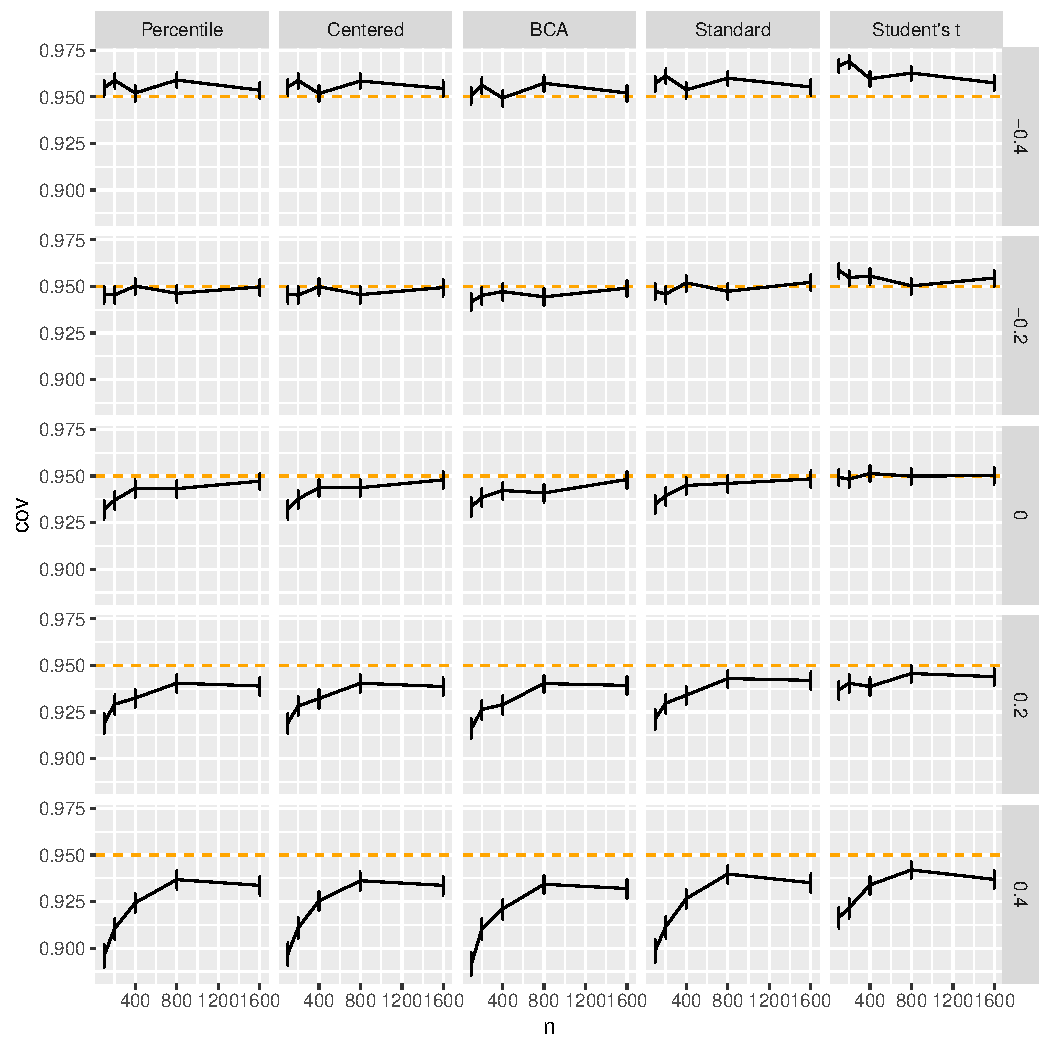
\includegraphics[width=\textwidth]{figures/plot_mu}
  \caption{Plots of $\mu$ coverage rates for each interval type and $\phi$
    combination. The orange dotted line represents the 95\% nominal coverage
    rate. The error bars represent a 95\% CI for the coverage
    proportion out of 10000 replications for each $n$. Results from $n$
    ranging from 100-700 were recorded.}
  \label{fig:mu}
\end{figure}


\begin{figure}[tbp]
  \centering
  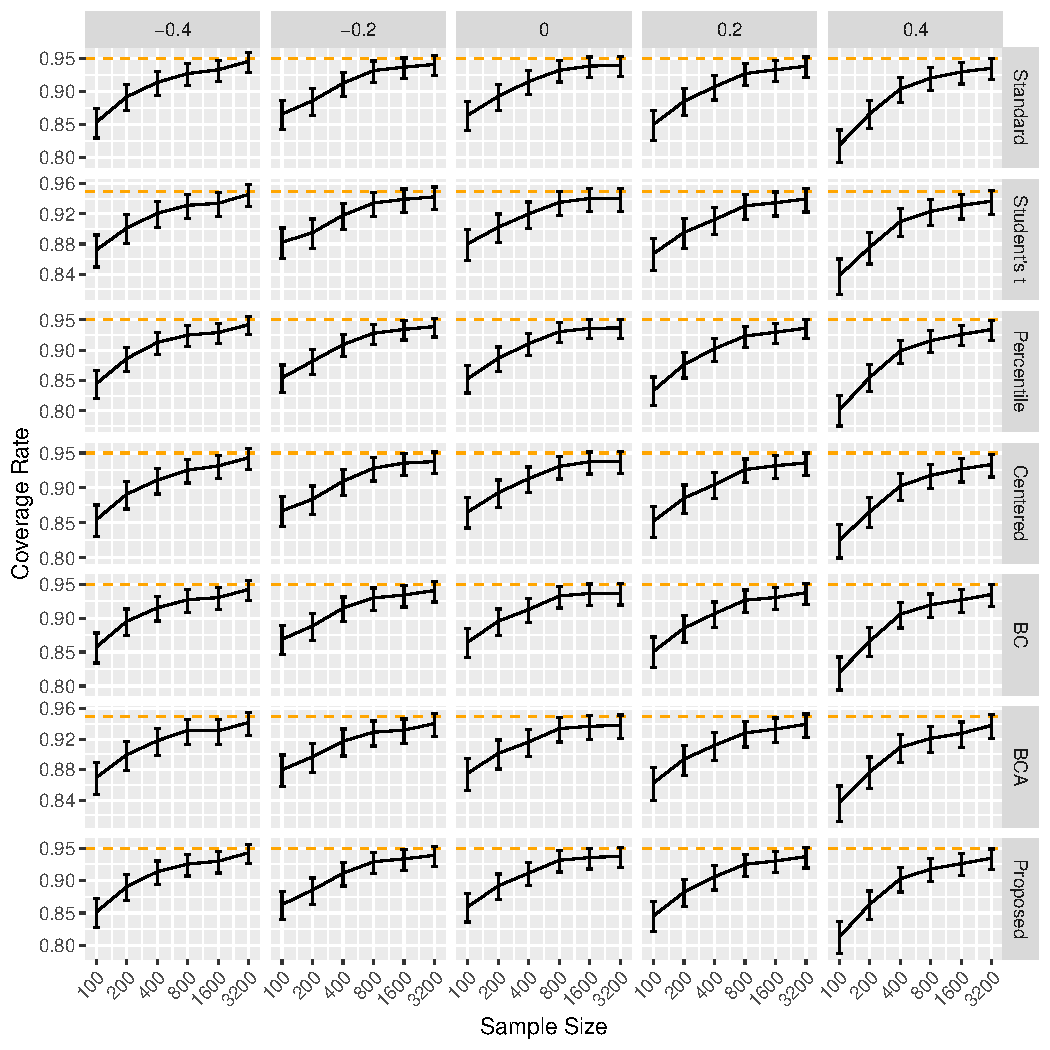
\includegraphics[width=\textwidth]{figures/plot_sigma}
  \caption{Plots of $\sigma$ coverage rates for each interval type and $\phi$
    combination. The orange dotted line represents the 95\% nominal coverage
    rate. The error bars represent a 95\% CI for the coverage
    proportion out of 10000 replications for each $n$. Results from $n$
    ranging from 100-700 were recorded.}
  \label{fig:sigma}
\end{figure}


\begin{figure}[tbp]
  \centering
  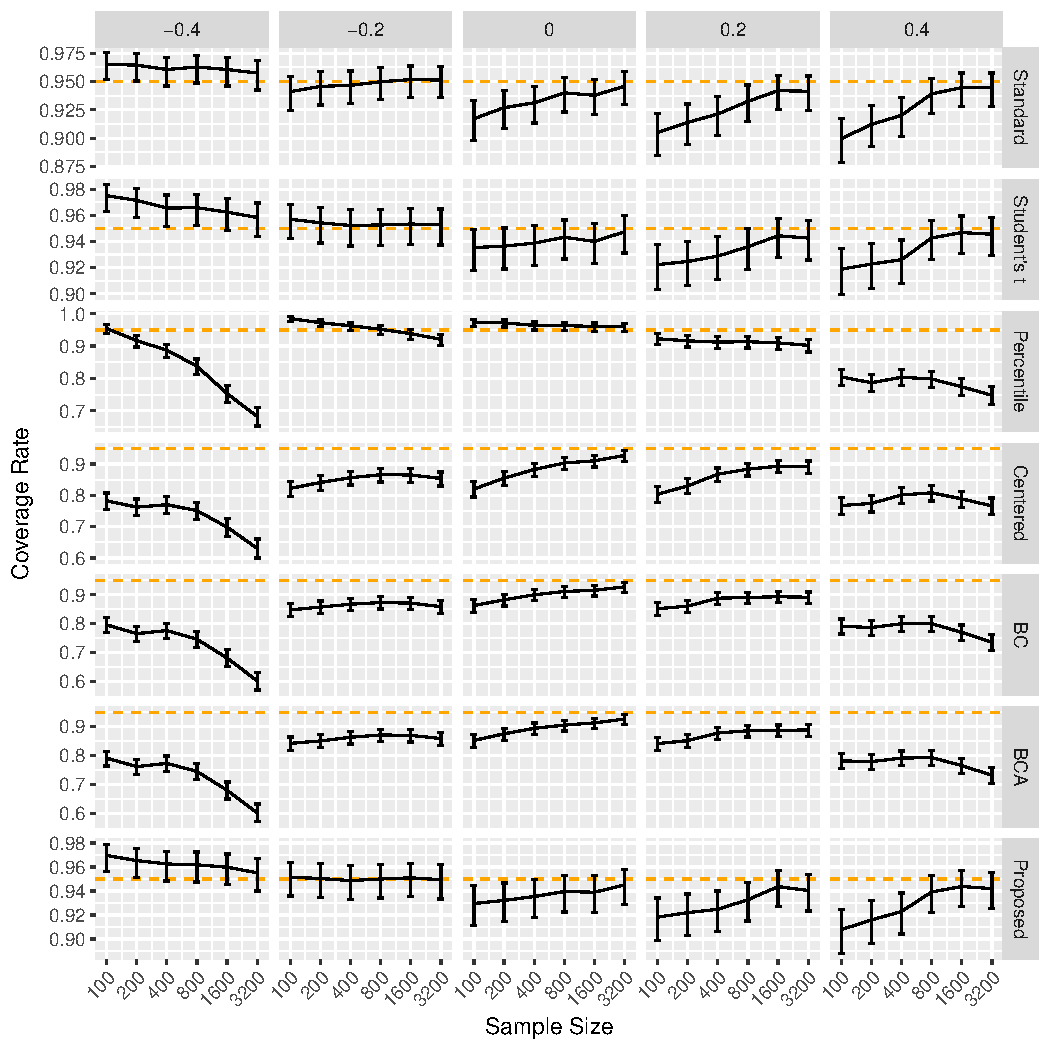
\includegraphics[width=\textwidth]{figures/plot_phi}
  \caption{Plots of $\phi$ coverage rates for each interval type and $\phi$
    combination. The orange dotted line represents the 95\% nominal coverage
    rate. The error bars represent a 95\% CI for the coverage
    proportion out of 10000 replications for each $n$. Results from $n$
    ranging from 100-700 were recorded.}
  \label{fig:phi}
\end{figure}


As shown in the above figures, only $\hat{\theta}_{n}$-centered intervals
managed to solve the deterioration problem with respect to recovering $\phi$,
indicating that this interval should be used as opposed to the uncentered
percentile interval or the more complex $BC_a$ interval when estimating
$\phi$. Increasing $n$ will not fix the performance of either of these
intervals because the assumption that the coverage rate will approach an upper
limit of .95 as $n$ increases is invalid. As expected for
$\hat{\theta}_{n}$-centered intervals, a higher positive $\phi$ demands a
larger $n$ to estimate all parameters, but a negative $\phi$ may require a
lesser $n$. For example, for both $\phi = 0.2$ and $0.4$, $n = 100$ was
sufficient to recover $\mu$ at a rate of approximately 95\%.


\section{Concluding Remarks}
\label{sec:conremarks}

\jy{Discussion points:
  1) common practice on block bootstrap even for simple parameter such as the
  mean;
  2) further investigation needed for phi;
  3) impact on applied statsitics courses; student reactions (Dr. Schifano).
}


Block bootstrap method is a useful method for estimating parameters of a time
series: from simple parameters like the mean to temporal dependence factors.
The motivation for the study is the idea that block bootstrap procedure will
perfectly estimate a parameter of a time series given an infinitely large
sample. The goal for this study was to find what is a good enough finite
sample length for block bootstrap estimation to recover the parameter of a
time series at an acceptable rate.


Again, this relies on the assumption that
there is a size $n$ large enough for the method to work: that is, the method's
performance improves as $n$ increases. Out of the two types of intervals used
in this study, this assumption was found to hold true with respect to
estimating $\phi$ only for $\hat{\theta}_{n}$-centered intervals, whereas both
percentile $BC_a$ intervals exhibited coverage deterioration as $n$
increased.


When using $\hat{\theta}_{n}$-centered intervals and $\phi$ is
unknown, the results of this study suggest that an $n$ of around 500 may be
necessary for common practice to estimate a simple parameter like $\mu$, and
an $n$ of around 400 may be necessary to
estimate $\sigma$. If $\phi$ is already known, a lesser $n$ may be adequate to
estimate these parameters. When $\phi$ was negative, a $n$ of around 100 was
sufficient to estimate $\mu$. However, in real world applications, $\phi$ is
more commonly found to be positive, so a larger $n$ is more likely to be
necessary. Lastly, to estimate $\phi$, an $n$ of around 400 may be necessary.
Further investigation may be necessary to see if there are other interval
corrections that fix the coverage deterioration problem for $\phi$.


This study could be used as a guide for applied statistics courses for students
to generally understand how large of a sample size is sufficient for block
bootstrap to be used versus other inference methods.
This information could prove to be useful for researching using block bootstrap
estimation of time series in domains such as econometrics. Future studies
could investigate if there are types of block bootstrap intervals
constructions that would more appropriately recover the parameters of a time
series. One could also investigate the $n$ needed to make inferences about
other forms of serially dependent data such as an MA process.


\bibliographystyle{chicago}
\bibliography{citations}

\end{document}

BBOB
B
